%%%%%%%%%%%%%%%%%%%%%%%%%%%%%%%%%%%%%%%%%
% Usability study
% Usability study of passenger information systems in Cracow
%
% Presentation for Usability Engineering
%
%%%%%%%%%%%%%%%%%%%%%%%%%%%%%%%%%%%%%%%%%

%----------------------------------------------------------------------------------------
%	PACKAGES AND THEMES
%----------------------------------------------------------------------------------------

\documentclass{beamer}

\usepackage[T1]{fontenc}
\usepackage[polish]{babel}
\usepackage[utf8]{inputenc}
\usepackage{lmodern}
\usepackage{amsmath}

\selectlanguage{polish}

\mode<presentation> {
	\usetheme{Copenhagen}
}

\usepackage{graphicx} % Allows including images
\usepackage{booktabs} % Allows the use of \toprule, \midrule and \bottomrule in tables


% Custom macros

\newcommand{\red}[1]{
	{ \color{red}{#1} }
}

\newcommand{\score}[2]{
	\stackrel
	{\red{#1}}
	{#2}
}

\definecolor{links}{HTML}{2A1B81}
\hypersetup{colorlinks,linkcolor=,urlcolor=links}


%----------------------------------------------------------------------------------------
%	TITLE PAGE
%----------------------------------------------------------------------------------------

\title
[Usability study of Passenger Information Systems]
{Usability study of Passenger Information Systems in Cracow Public Transport}

\author
[M.Salawa, J. Stępak]
{Małgorzata Salawa, \ Jakub Stępak}

\institute
[AGH]
{
AGH University of Science and Technology

}
\date{7th November 2016}

%----------------------------------------------------------------------------------------

\begin{document}

\frame{\titlepage}

%----------------------------------------------------------------------------------------
%	PRESENTATION SLIDES
%----------------------------------------------------------------------------------------

%------------------------------------------------
\section{Usability study}
%------------------------------------------------

\subsection{Object of usability study}

\begin{frame}

\frametitle{Passenger Information System (PIS)}
\begin{center}

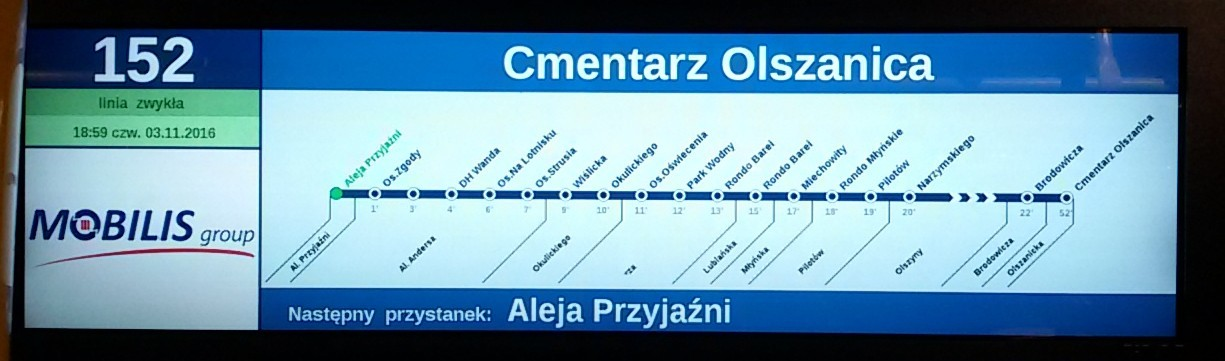
\includegraphics[width=0.8\paperwidth]{sip1.jpg}

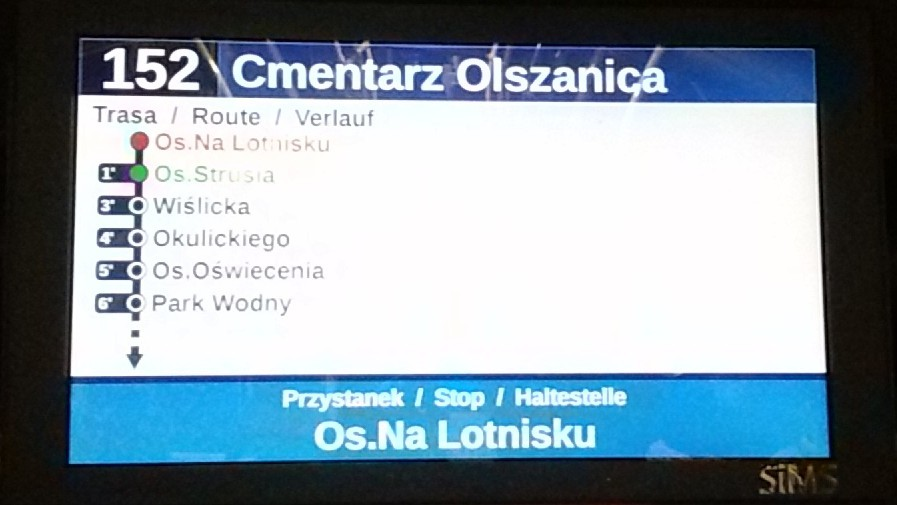
\includegraphics[width=0.4\paperwidth]{sip2.jpg}

\end{center}

\end{frame}

%------------------------------------------------

\subsection{Planned method}

\begin{frame}
\frametitle{Planned method}

\begin{itemize}
\item Online survey
\end{itemize}

\end{frame}

%------------------------------------------------

\subsection{Other remarks}

\begin{frame}
\frametitle{Other remarks}

Considering that many people use Public Transport in daily basis, we believe that reaching users should be easy.
There are also groups and pages on Facebook that we can use to spread out link to survey.

\end{frame}

%------------------------------------------------

\end{document} 
